\documentclass[]{article}
\usepackage[colorlinks=true,urlcolor=blue]{hyperref}
\usepackage{graphicx}
\usepackage{sidecap}
\setlength{\parindent}{0em}
\setlength{\parskip}{1em}
\begin{document}

\title{Not your normal chromosome 10}
\maketitle

Chromsomal knob are one of my favorite things about maize. Knobs are large regions of heterochromatin, made up of short tandem repeats that can span many, many, megabases.  They are easily seen through a microscope:

%\begin{SCfigure}[][h!]   
%   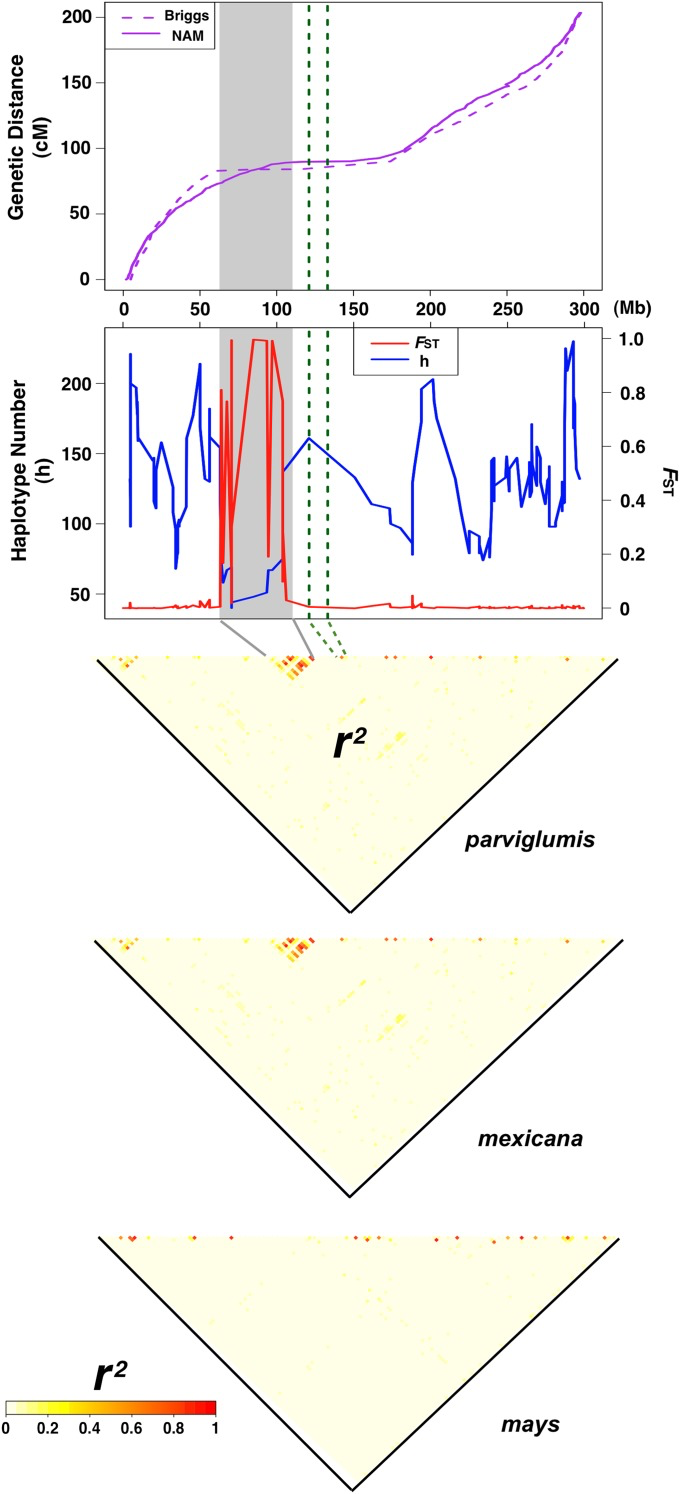
\includegraphics[width=0.3\linewidth]{/Users/jri/gdrive/fruitcase/883fig1.png}
%   \caption{The impact of an inversion on diversity. Figure from \href{http://www.genetics.org/content/191/3/883}{Fang et al. 2012} showing reduced haplotype diversity, elevated $F_{ST}$ between haplotypes, increased LD, and decreased rates of crossover inside a large inversion on maize chromosome 1.} 
%    \label{fig:fang}
%\end{SCfigure}

%\begin{figure*}[h]   
%  \begin{center}
%   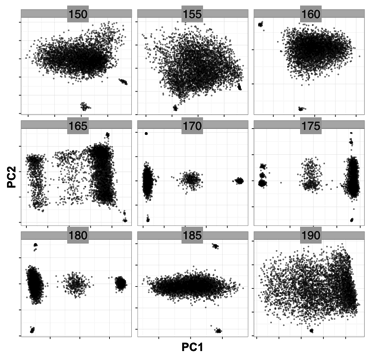
\includegraphics[width=0.7\linewidth]{/Users/jri/gdrive/fruitcase/inversions_pca.png}
%   \caption{ The first two principal components of a PCA on individuals from the maize SeeDs of diversity data, plotted in 5Mb windows for part of Chr. 4. You can see a high-res version at the 1Mb scale \href{}{here}.} 
%    \label{fig:pcs}
%  \end{center}
%\end{figure*}

\end{document}